\documentclass[a4paper]{article}

%% Language and font encodings
\usepackage[english]{babel}
\usepackage[utf8x]{inputenc}
\usepackage[T1]{fontenc}

%% Sets page size and margins
\usepackage[a4paper,top=3cm,bottom=2cm,left=3cm,right=3cm,marginparwidth=1.75cm]{geometry}

%% Useful packages
\usepackage{amsmath}
\usepackage{amsfonts}
\usepackage{amssymb}
\usepackage{graphicx}
\usepackage{subcaption}
\usepackage[colorinlistoftodos]{todonotes}
\usepackage[colorlinks=true, allcolors=blue]{hyperref}

\graphicspath{ {figures/} }

% Commands
\newcommand{\alphabet}{\mathcal{A}}
\newcommand{\fullAlignment}{\mathbf{Y}}
\newcommand{\alignmentColumn}{\mathbf{y}}
\newcommand{\sitePattern}{s}
\newcommand{\siteSplit}{S'}
\newcommand{\sitePatternSet}{S}
\newcommand{\fullSitePatterns}{\mathbf{s}}
\newcommand{\sitePatternSpace}{\mathcal{S}}
\newcommand{\fullAncestralStates}{\mathbf{H}}
\newcommand{\ancestralStateSpace}{\mathcal{H}}
\newcommand{\ancestralStateColumn}{\boldsymbol\eta}
\newcommand{\ancestralStateCategory}{Z}
\newcommand{\ancestralSplit}{H'}
\newcommand{\ancestralStateSet}{H}
\newcommand{\fullAncestralStateCategories}{\mathbb{Z}}
\newcommand{\ancestralStateCategorySpace}{\mathcal{Z}}

\newcommand{\nCols}{n}
\newcommand{\nSiteRows}{m}
\newcommand{\nAncestralStateRows}{p}
\newcommand{\nSiteSplits}{q}
\newcommand{\nAncestralSplits}{r}
\newcommand{\nMostLikelyAncestralSplits}{\tilde{r}}


\title{Possible Inconsistency in Maximum Likelihood Calculation of Ancestral States}
\author{Shaw, Matsen, Minin}

\begin{document}
\maketitle

%comments from Erick:
% >  This is great!
% > - would be great to have all the calculations showing the "refinement" structure written out for the various tree structures (just done by hand and scanned is just fine)
% > - I think of the "refinement" as a partition, so perhaps rather than "empty refinement" we have a "single-element partition"
% > - in order to interpret the site patterns I need to figure out in what order the leaves are labeled
% > - how is ell calculated?
% > - on the numerical sanity check, it doesn't seem clear that the branch lengths can be different than the inferred ones-- they can!
% > - re "general case", agreed though I don't think that we need numerical optimization of branch lengths in a set of a branch length partition-- we can just get the optimal branch length directly. Namely, for each branch, we know all hidden states (given that we are in a set of a partition) and so can count the number of mutations across that branch. From there we have a simple likelihood function, which either has an optimal in the interior or on the boundary of the partition.

\renewcommand{\arraystretch}{1.2} % because otherwise exponents get eaten by \hline


\section*{Introduction}

Classical maximum-likelihood (ML) estimation in phylogenetics operates by integrating out possible ancestral states at the internal nodes of the tree.
Recently \cite{Neher2017} have suggested using an approximation to ML inference in which the likelihood is maximized jointly across model parameters and ancestral sequences.
This is attractive from a computational perspective: joint ML inference can proceed according to an iterative procedure in which ML ancestral sequences are first inferred and then model parameters are optimized conditional on the ancestral sequences.
% I would say classical maximum likelihood is closer to EM, no? At some point in EM we'd have to marginalize/take the expectation, which joint ML doesn't do. Curious to talk more about it though...
This latter step is much simpler and more computationally efficient when conditioning on ancestral sequences compared to the case in which ancestral sequences are marginalized out.

However, existing consistency proofs for phylogenetics \cite{RoyChoudhury2015-ta} do not apply to the setting of joint inference of trees and ancestral sequences.
There are examples in statistics, such as the Neyman-Scott paradox \cite{Neyman1948-tt}, in which estimation of additional parameters destroys consistency.
This raises the question of whether joint inference of trees and ancestral sequences enjoys good statistical properties.

In this paper we show that the joint inference of trees and ancestral sequences is not consistent in general.
To do so, we follow a strategy of using simple models and four taxa trees.
Here we use a binary symmetric model and simulate on the ``Farris zone'' \cite{Siddall1998-hq} tree.
We use bounds on the joint likelihood to demarcate a sizeable area of long branch lengths in which joint inference converges on the wrong tree.

\section{Ancestral state reconstruction using maximum likelihood}

We will be considering phylogenetic likelihood on unrooted phylogenetic trees.
We assume the character alphabet $\alphabet=\{0,1\}$ and a uniform stationary distribution.
Let $\nSiteRows$ be the number of tips of the tree, and $\nAncestralStateRows = \nSiteRows-2$ the number of internal nodes.
%EM Commented out below because it's not right-- fullAlignment is not the set of assignments of characters to tips of the tree, it's a single such.
%Let $\fullAlignment$ be the set of assignments of characters to tips of our tree, and $\fullAncestralStates$ the set of assignments of characters to the internal nodes of the tree.
Assume we observe $\nCols$ samples of character data (i.e.\ an alignment with $\nCols$ columns) $\fullAlignment=[\alignmentColumn_1,\ldots,\alignmentColumn_\nCols]\in\alphabet^{\nSiteRows\times\nCols}$.
There are also corresponding unknown ancestral states $\fullAncestralStates=[\ancestralStateColumn_1,\ldots,\ancestralStateColumn_\nCols]\in\alphabet^{\nAncestralStateRows\times\nCols}$.

\subsection{Classical maximum-likelihood inference in phylogenetics}

For a topology $\tau$ and branch lengths $t$ we form the fully-observed likelihood (making the usual independence assumption between sites):
\begin{equation}
\label{eq:full_likelihood}
L_\nCols(\fullAlignment;\fullAncestralStates, \tau, t) = \prod_{i=1}^{\nCols} \ P(\alignmentColumn_i, \ancestralStateColumn_i | \tau, t).
\end{equation}
% In particular, we are interested in
% $$
% (\hat{\boldsymbol\xi}, \hat{\tau}, \hat{t}) = \arg\max_{\boldsymbol\xi, \tau, t} \ L_n(\mathbf{y};\boldsymbol\xi, \tau, t),
% $$
% which we call the maximum likelihood values of the parameters $(\boldsymbol\xi, \tau, t)$.
% Since the number of elements in $\boldsymbol\xi$ grows with that of the observed data $\mathbf{y}$,
The typical approach to estimate the tree $\tau$ and branch lengths $t$ involves computing the marginal likelihood
\begin{equation}
\label{eq:marginal_likelihood}
\tilde{L}_\nCols(\fullAlignment; \tau, t) = \sum_{\fullAncestralStates} \ L_\nCols(\fullAlignment;\fullAncestralStates, \tau, t)
\end{equation}
and maximizing over the topology and branch lengths to obtain
$$
(\hat{\tau}, \hat{t}) = \arg\max_{\tau, t} \  \tilde{L}_\nCols(\fullAlignment; \tau, t).
$$
% The values $\hat{\boldsymbol\xi}$ are then calculated conditional on these estimates.
% More likely in practice we fix a topology $\tau$ and use this marginalization approach to compute $(\hat{\boldsymbol\xi}, \hat{t})$.

\subsection{Joint maximization}

One tantalizing approach is to do away with the marginalization and directly estimate the maximum likelihood parameters from the full likelihood in \eqref{eq:full_likelihood}.
We can perform this by computing the profile likelihood
\begin{equation}
\label{eq:profile_likelihood}
L_\nCols'(\fullAlignment;\tau, t) = \max_{\fullAncestralStates} \ L_\nCols(\fullAlignment;\fullAncestralStates, \tau, t),
\end{equation}
then estimating the topology and branch lengths via
\begin{equation}
\label{eq:profile_likelihood_topology_bl}
(\hat{\tau}, \hat{t}) = \arg\max_{\tau, t} \ L_\nCols'(\fullAlignment;\tau, t)
\end{equation}
while using $\hat{\fullAncestralStates}$ maximizing \eqref{eq:profile_likelihood} as an estimate for $\fullAncestralStates$.
Since $\alphabet$ is a discrete set, there exists a maximum \eqref{eq:profile_likelihood}, and so \eqref{eq:profile_likelihood_topology_bl} will recover the joint ML values of the unknown parameters.
In the general case, the functional form of \eqref{eq:profile_likelihood} is determined by inequalities that depend on the unknown $(\tau,t)$.
For this reason, in practice the joint ML strategy estimates $\hat{\fullAncestralStates}$ for a fixed $(\tau,t)$, then $(\hat{\tau},\hat{t})$ given $\hat{\fullAncestralStates}$, maximizing each of these conditional objectives until convergence \cite{Neher2017}.

\subsection{Site split formulation}

Since we have a finite character alphabet, for a given column $i$ there are a finite number of possibilities of assignments of characters to tips $\alignmentColumn_i$ or internal nodes $\ancestralStateColumn_i$.
Following Section 8.6 of \cite{Semple2003}, $\tau$ induces an ordered set of tip labels $\{1,\ldots,\nSiteRows\}$ across sites.
For a binary character model, a realization of $\alignmentColumn_i$ can be described as a subset of complementary characters $\siteSplit\subseteq\sitePatternSet\triangleq\{1,\ldots,\nSiteRows-1\}$.
The topology $\tau$ induces an ordered set $\{1,\ldots,\nAncestralStateRows\}$ for $\ancestralStateColumn_i$ with a similar subset of complementary characters $\ancestralSplit\subseteq\ancestralStateSet\triangleq\{1,\ldots,\nAncestralStateRows\}$ describing a realization of $\ancestralStateColumn_i$.
Define the total number of unique site splits as $\nSiteSplits=|\mathcal{P}(\sitePatternSet)|$ and unique ancestral state splits as $\nAncestralSplits=|\mathcal{P}(\ancestralStateSet)|$ where $\mathcal{P}$ denotes the powerset.

%EM in general aren't a different number of internal site patterns than tip site patterns?
%das: Yes, I moved the paragraph at the end to here so it's hopefully less confusing. Maybe writing out the example would help? I also changed from "pattern" to "category" which might make it a little more clear.
%EM Seems good this is an important concept so it's worth defining it more properly.

Consider the probability $P(\alignmentColumn_i, \ancestralStateColumn_i | \tau, t)$ from \eqref{eq:full_likelihood} of observing a particular column $i$.
Given $(\tau, t)$ and maximizing over $\ancestralStateColumn_i$, if $\alignmentColumn_i=\siteSplit_j$ then there exists a partition $\ancestralStateCategory_j$ of $\mathcal{P}(\ancestralStateSet)$ of most likely ancestral states where
\begin{align*}
\max_{\ancestralSplit_k\in\mathcal{P}(\ancestralStateSet)} \ P(\alignmentColumn_i=\siteSplit_j, \ancestralStateColumn_i=\ancestralSplit_k | \tau, t) &= P(\alignmentColumn_i=\siteSplit_j, \ancestralStateColumn_i\in\ancestralStateCategory_j | \tau, t) \\
     &= P(\alignmentColumn=\siteSplit_j, \ancestralStateColumn\in\ancestralStateCategory_j | \tau, t).
\end{align*}
This equivalence is helpful in writing the full likelihood of the joint inference problem in terms of site splits; for most likely ancestral state partitions $\fullAncestralStateCategories=\{\ancestralStateCategory_1,\ldots,\ancestralStateCategory_\nSiteSplits\}$ we reformulate the likelihood equation
\begin{align}
L_\nCols'(\fullAlignment;\tau, t) &= \max_{\fullAncestralStates} \ L_\nCols(\fullAlignment;\fullAncestralStates, \tau, t) \\
                             &= \max_{\fullAncestralStates} \ \prod_{i=1}^{\nCols} \ P(\alignmentColumn_i, \ancestralStateColumn_i | \tau, t) \\
                             &= \prod_{i=1}^{\nCols} \ \max_{\ancestralSplit_k\in\mathcal{P}(\ancestralStateSet)} \ P(\alignmentColumn_i=\siteSplit_j, \ancestralStateColumn_i=\ancestralSplit_k | \tau, t) \\
%EM Can you think a little about z_j?
%EM Even though it's a category now, it's still a function of tau and t, right?
                             &= \prod_{i=1}^{\nCols} \ P(\alignmentColumn=\siteSplit_j, \ancestralStateColumn\in\ancestralStateCategory_j | \tau, t) \\
                             &= \prod_{j=1}^{\nSiteSplits} \ P(\alignmentColumn=\siteSplit_j, \ancestralStateColumn\in\ancestralStateCategory_j | \tau, t)^{\nCols_j(\fullAlignment)} \label{eq:site_pattern_likelihood}
\end{align}
where $\nCols_j(\fullAlignment)$ is the number of columns in $\fullAlignment$ where the site split $\siteSplit_j$ appears.

\subsection{Showing inconsistency}

We are interested in the properties of the objective function being maximized in \eqref{eq:site_pattern_likelihood} as data becomes plentiful.
Define \eqref{eq:site_pattern_likelihood} as
$$
L_\nCols''(\fullAlignment;\fullAncestralStateCategories,\tau,t) = \prod_{j=1}^{\nSiteSplits} \ P(\alignmentColumn=\siteSplit_j, \ancestralStateColumn\in\ancestralStateCategory_j | \tau, t)^{\nCols_j(\fullAlignment)} .
$$
Assume our $\nCols$ observations were generated from a model with parameters $(\tau^*, t^*)$.
We have
\begin{align}
    \frac{1}{\nCols} \log L_\nCols''(\fullAlignment;\fullAncestralStateCategories,\tau,t)
        &= \sum_{j}^\nSiteSplits \frac{\nCols_j(\fullAlignment)}{\nCols}\cdot  \log P(\alignmentColumn=\siteSplit_j, \ancestralStateColumn\in\ancestralStateCategory_j | \tau, t) \\
        &= \sum_{j}^\nSiteSplits \frac{\nCols_j(\fullAlignment)}{\nCols}\cdot [\log P(\alignmentColumn=\siteSplit_j | \tau, t) + 
            \log P(\ancestralStateColumn\in\ancestralStateCategory_j | \alignmentColumn=\siteSplit_j , \tau, t)]
\end{align}
so that, in the limit of infinite data,
\begin{equation}
\frac{1}{\nCols} \log L_\nCols''(\fullAlignment;,\tau,t) \rightarrow \sum_{j}^\nSiteSplits P(\alignmentColumn=\siteSplit_j | \tau^*, t^*) \cdot [\log P(\alignmentColumn=\siteSplit_j | \tau, t) + \log P(\ancestralStateColumn\in\ancestralStateCategory_j | \alignmentColumn=\siteSplit_j , \tau, t)]. \label{eq:site_pattern_profile_likelihood_mean}
\end{equation}
Define the the information quantity
$$
h_{\tau^*,t^*}(\tau,t) = \sum_{j}^\nSiteSplits P(\alignmentColumn=\siteSplit_j | \tau^*, t^*) \log P(\siteSplit_j | \tau, t),
$$
and the partial log likelihood
$$
\ell^p_{\tau^*,t^*}(\fullAncestralStateCategories,\tau,t) = \sum_{j}^\nSiteSplits P(\alignmentColumn=\siteSplit_j | \tau^*, t^*) \log P(\ancestralStateColumn\in\ancestralStateCategory_j | \siteSplit_j, \tau, t)
$$
so that \eqref{eq:site_pattern_profile_likelihood_mean} is written as
\begin{equation}
    \label{eq:log_likelihood_simplified}
\ell_{\tau^*,t^*}(\fullAncestralStateCategories,\tau,t) = h_{\tau^*,t^*}(\tau,t) + \ell^p_{\tau^*,t^*}(\fullAncestralStateCategories,\tau,t).
\end{equation}
Recall $(\tau, t)$ are estimands and $(\tau^*, t^*)$ are fixed, generating parameters.
For data generated from $(\tau^*, t^*)$, if
\begin{equation}
\label{eq:inconsistency_inequality}
\ell_{\tau^*,t^*}(\hat{\fullAncestralStateCategories}_1,\tau',\hat{t}_1) > \ell_{\tau^*,t^*}(\hat{\fullAncestralStateCategories}_2,\tau^*,\hat{t}_2)
\end{equation}
for $\tau'\neq\tau^*$ with $\{\hat{t}_1,\hat{\fullAncestralStateCategories}_1\}$ and $\{\hat{t}_2,\hat{\fullAncestralStateCategories}_2\}$ estimated by maximizing \eqref{eq:profile_likelihood}, we have an inconsistency.

\section{Inconsistency of joint maximum likelihood}

\subsection{Bounding the likelihoods}

Our approach will be to seek bounds for the terms inside the maximization in \eqref{eq:log_likelihood_simplified} as
\begin{equation}
\label{eq:partial-likelihood}
\ell_{\tau^*,t^*}(\fullAncestralStateCategories,\tau,t) = h_{\tau^*,t^*}(\tau,t) + \ell^p_{\tau^*,t^*}(\fullAncestralStateCategories,\tau,t).
\end{equation}
We obtain an upper bound for the joint maximum of \eqref{eq:partial-likelihood}
$$
\max_{t,\fullAncestralStateCategories} \ \ell_{\tau^*,t^*}(\fullAncestralStateCategories,\tau,t) \le
    h_{\tau^*,t^*}(\tau^*,t^*)
    + \ell^p_{\tau^*,t^*}(\hat{\fullAncestralStateCategories},\tau,\hat{t})
$$
using Gibbs's inequality
$$
h_{\tau^*,t^*}(\tau,t) \le h_{\tau^*,t^*}(\tau^*,t^*)
$$
and
$$
\{\hat{t},\hat{\fullAncestralStateCategories}\} = \arg\max_{t,\fullAncestralStateCategories} \ \ell^p_{\tau^*,t^*}(\fullAncestralStateCategories,\tau,t).
$$
Similarly, we have a lower bound as
$$
\max_{t,\fullAncestralStateCategories} \ \ell_{\tau^*,t^*}(\fullAncestralStateCategories,\tau,t) \ge
    h_{\tau^*,t^*}(\tau,\hat{t})
    + \ell^p_{\tau^*,t^*}(\hat{\fullAncestralStateCategories},\tau,\hat{t}).
$$

% vvvv Remove these? I think they're obvious now, but maybe they can be made more explicit above?
\textbf{Argument for lower bound}: This makes intuitive sense, though may be difficult to show in general.
Can we not just say $\max_u f(u) + g(u)$ is greater than $f(u') + g(u')$ for any $u'$ that doesn't maximize $f(u) + g(u)$ just by definition?
There could be multiple maxima, but that's why we have greater than or equal to.
I think the only thing we'd need to show is that a maximum exists, but since $\{x,y,w\}$ are supported on a closed set this is certainly true.
I must be missing something.

\textbf{Argument for upper bound}: I think this is true mostly because $\max_u f(u) + g(u)$ should be less than $\max_u f(u) + \max_u g(u)$ by some triangle inequality argument.
If we were to actually maximize the full likelihood, we should get something smaller than maximizing some form of it that we consider by looking at the parts separately.
For a fixed $\{x^*, y^*\}$ we can calculate this upper bound directly---can we obtain it as a useful-looking function of these parameters in the general case?

\subsection{Parameter setting}

\begin{figure}
\centering
\begin{subfigure}{.45\linewidth}
\centering
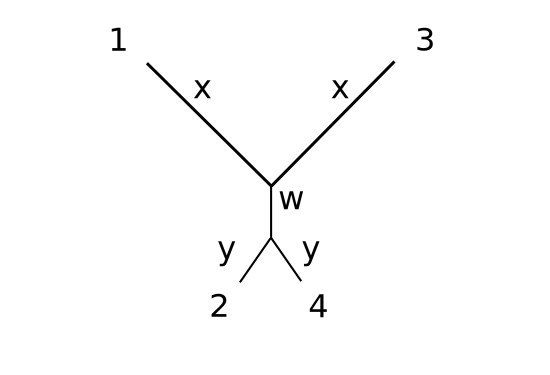
\includegraphics[width=.95\textwidth]{farris_blank}
\caption[short]{Farris topology $\tau_1$}
\end{subfigure}
\begin{subfigure}{.45\linewidth}
\centering
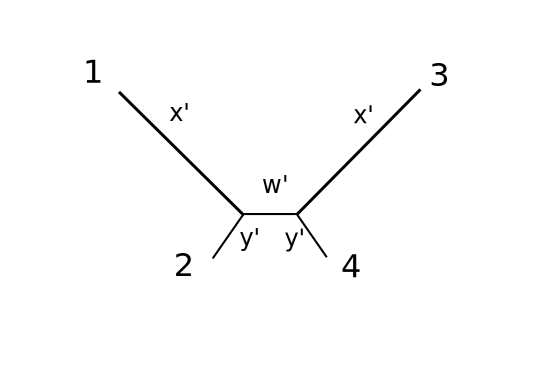
\includegraphics[width=.95\textwidth]{felsenstein_blank}
\caption[short]{Felsenstein topology $\tau_2$}
\end{subfigure}
\caption{Two simple topologies}
\label{fig:farris-fels-top}
\end{figure}

Define the Farris topology $\tau_1$ and the Felsenstein topology $\tau_2$ as in Figure~\ref{fig:farris-fels-top}.
Call $t=\{x,y,w\}$ and $t^*=\{x,y,y\}$, i.e., $t^*$ is the case where the bottom three branches all share the same parameter, the classical construction of this topology.
The branch length parameters are such that the probability of a change in character along the top two branches is $p_x=1-2x$, with corresponding equalities for the other two branches.
Here, $\{p_x,p_y,p_w\}\in[0,1/2]^3$ and $\{x,y,w\}\in[0,1]^3$.

\textbf{Justification for estimand:} It might be worth arguing why this form of the estimand $t$ is necessary.
I think the idea is that for either of these topologies, any maximum obtained will occur where the top two and bottom two branches are equal, though not necessarily the middle branch.
This would be good to show explicitly.

Table~\ref{tab:sitepatprob} contains calculations of site pattern frequencies under these two topologies, calculated using the Hadamard transform approach outlined in 8.6 of Semple and Steel \cite{Semple2003-em}.
Table~\ref{tab:likelihoods} contains calculations of likelihood values for fixed site patterns and topologies, with the maximum values over ancestral state patterns noted.

\begin{table}
\centering
\begin{tabular}{|l|l|l|}
\multicolumn{3}{c}{Classical}\\
    \hline
$\siteSplit_j$   &$P(\alignmentColumn=\siteSplit_j|\tau_1,t^*)$&$P(\alignmentColumn=\siteSplit_j|\tau_2,t^*)$\\
    \hline
    $\{\emptyset\}$&$1+x^2+y^2+4xy^2+x^2y^2$&$1+2xy+2xy^2+x^2y+y^3+x^2y^2$\\
    $\{1\}$        &$1-x^2+y^2-x^2y^2$&$1-x^2y+y^3-x^2y^2$\\
    $\{2\}$        &$1+x^2-y^2-x^2y^2$&$1+x^2y-y^3-x^2y^2$\\
    $\{3\}$        &$1-x^2+y^2-x^2y^2$&$1-x^2y+y^3-x^2y^2$\\
    $\{1,2\}$      &$1-x^2-y^2+x^2y^2$&$1+2xy-2xy^2-x^2y-y^3+x^2y^2$\\
    $\{1,3\}$      &$1+x^2+y^2-4xy^2+x^2y^2$&$1-2xy-2xy^2+x^2y+y^3+x^2y^2$\\
    $\{2,3\}$      &$1-x^2-y^2+x^2y^2$&$1-2xy+2xy^2-x^2y-y^3+x^2y^2$\\
    $\{1,2,3\}$    &$1+x^2-y^2-x^2y^2$&$1+x^2y-y^3-x^2y^2$\\
    \hline
\multicolumn{3}{c}{Modified}\\
    \hline
$\siteSplit_j$   &$P(\alignmentColumn=\siteSplit_j|\tau_1,t)$&$P(\alignmentColumn=\siteSplit_j|\tau_2,t)$\\
    \hline
    $\{\emptyset\}$&$1+x^2+y^2+4xyw+x^2y^2$&$1+2xy+2xyw+x^2w+y^2w+x^2y^2$\\
    $\{1\}$        &$1-x^2+y^2-x^2y^2$&$1-x^2w+y^2w-x^2y^2$\\
    $\{2\}$        &$1+x^2-y^2-x^2y^2$&$1+x^2w-y^2w-x^2y^2$\\
    $\{3\}$        &$1-x^2+y^2-x^2y^2$&$1-x^2w+y^2w-x^2y^2$\\
    $\{1,2\}$      &$1-x^2-y^2+x^2y^2$&$1+2xy-2xyw-x^2w-y^2w+x^2y^2$\\
    $\{1,3\}$      &$1+x^2+y^2-4xyw+x^2y^2$&$1-2xy-2xyw+x^2w+y^2w+x^2y^2$\\
    $\{2,3\}$      &$1-x^2-y^2+x^2y^2$&$1-2xy+2xyw-x^2w-y^2w+x^2y^2$\\
    $\{1,2,3\}$    &$1+x^2-y^2-x^2y^2$&$1+x^2w-y^2w-x^2y^2$\\
    \hline
\end{tabular}
\caption{Site pattern probabilities.
All values are multiplied by $1/8$.}
\label{tab:sitepatprob}
\end{table}

\begin{table}
\centering
\begin{tabular}{|l|ll|}
    \multicolumn{3}{c}{$\tau=\tau_1$}\\
    \hline
    $\siteSplit_j$    & $\ancestralStateCategory_j$ & $P(\ancestralStateColumn\in\ancestralStateCategory_j|\alignmentColumn=\siteSplit_j,\tau,t)$\\
    \hline
    $\{\emptyset\}$&
    $\{\emptyset\}$&
    $(1+x)^2   (1+w)(1+y)^2$\\
     $\{1\}$    &
    $\{\emptyset\}$&
    $(1+x)(1-x)(1+w)(1+y)^2$\\
     $\{2\}$    &
    $\{\emptyset\}$&
    $(1+x)(1-x)(1+w)(1+y)^2$\\
     $\{3\}$    &
    $\{\emptyset\}$&
    $(1+x)^2   (1+w)(1+y)(1-y)$\\
    $\{1,2\}$  &
    $\{\{\emptyset\},\{1,2,3\}\}$&
    $(1+x)(1-x)(1+w)(1+y)(1-y)$\\
    $\{1,3\}$  &
    $\left\{\begin{array}{l}
                    \{\emptyset\}\\
                    \{2\}\\
                    \{1,2\}
                \end{array}\right.$&
    $\begin{array}{l}
                    (1+x)^2   (1+w)(1-y)^2\\
                    (1+x)^2   (1-w)(1+y)^2\\
                    (1-x)^2   (1+w)(1+y)^2
                \end{array}$\\
    $\{2,3\}$  &
                $\{\{\emptyset\},\{1,2,3\}\}$&
                $(1+x)(1-x)(1+w)(1+y)(1-y)$\\
    $\{1,2,3\}$&
                $\{\emptyset\}$&
                $(1+x)^2   (1+w)(1+y)(1-y)$\\
    \hline
    \multicolumn{3}{c}{$\tau=\tau_2$}\\
    \hline
    $\siteSplit_j$    & $\ancestralStateCategory_j$ & $P(\ancestralStateColumn\in\ancestralStateCategory_j|\alignmentColumn=\siteSplit_j,\tau,t)$\\
    \hline
    $\{\emptyset\}$       &$\{\emptyset\}$&$(1+x)^2   (1+w)(1+y)^2$\\
    $\{1\}$          &
    $\left\{\begin{array}{l}
                    \{\emptyset\}\\
                    \{1\}
                \end{array}\right.$&
    $\begin{array}{l}
                        (1+x)(1-x)(1+w)(1+y)^2\\
                        (1+x)^2   (1-w)(1+y)(1-y)
                    \end{array}$\\
      $\{2\}$          &
    $\left\{\begin{array}{l}
                    \{\emptyset\}\\
                    \{1\}
                \end{array}\right.$&
    $\begin{array}{l}
                    (1+x)^2   (1+w)(1+y)(1-y)\\
                    (1+x)(1-x)(1-w)(1+y)^2
                    \end{array}$\\
      $\{3\}$          &
    $\left\{\begin{array}{l}
                    \{\emptyset\}\\
                    \{2\}
                \end{array}\right.$&
    $\begin{array}{l}
                    (1+x)(1-x)(1+w)(1+y)^2\\
                    (1+x)^2   (1-w)(1+y)(1-y)
                    \end{array}$\\
     $\{1,2\}$         &
    $\left\{\begin{array}{l}
                    \{\{\emptyset\},\{1,2\}\}\\
                    \{2\}
                \end{array}\right.$&
    $\begin{array}{l}
                    (1+x)(1-x)(1+w)(1+y)(1-y)\\
                    (1+x)^2   (1-w)(1+y)^2
                    \end{array}$\\
     $\{1,3\}$         &
    $\left\{\begin{array}{l}
                    \{\emptyset\}\\
                    \{\{1\},\{2\}\}\\
                    \{1,2\}
                \end{array}\right.$&
    $\begin{array}{l}
                    (1+x)^2   (1+w)(1-y)^2\\
                    (1+x)(1-x)(1-w)(1+y)(1-y)\\
                    (1-x)^2   (1+w)(1+y)^2
                    \end{array}$\\
      $\{2,3\}$        &
    $\left\{\begin{array}{l}
                    \{\{\emptyset\},\{1,2\}\}\\
                    \{1\}\\
                    \{2\}
                \end{array}\right.$&
    $\begin{array}{l}
                    (1+x)(1-x)(1+w)(1+y)(1-y)\\
                    (1-x)^2   (1-w)(1+y)^2\\
                    (1+x)^2   (1-w)(1-y)^2
                    \end{array}$\\
     $\{1,2,3\}$       &
    $\left\{\begin{array}{l}
                    \{\emptyset\}\\
                    \{2\}
                \end{array}\right.$&
    $\begin{array}{l}
                    (1+x)^2   (1+w)(1+y)(1-y)\\
                    (1+x)(1-x)(1-w)(1+y)^2
                    \end{array}$\\
    \hline
\end{tabular}
\caption{Likelihood calculations for all site patterns and ancestral state categories.
All values multiplied by $1/32$.
Likelihoods with multiple entries will have maxima determined by unknown branch length parameters.}
\label{tab:likelihoods}
\end{table}

\subsubsection{Upper bound for Farris partial likelihood}

Assume $\tau^*=\tau_1$ and $t^*=\{x,y,y\}$.
Define, e.g., $p_0 = P(\alignmentColumn=\{\emptyset\}|\tau=\tau_1,t=\{x,y,y\})$.
Let
$$
    a_{0} = p_{13},
$$
$$
    a_{1} = p_1+p_2+p_{12}+p_{23},
$$
$$
    a_{2} = p_3+p_{12}+p_{23}+p_{123},
$$
$$
    a_{3} = p_1+p_3+p_{12}+p_{23},
$$
$$
    a_{4} = p_2+p_{12}+p_{23}+p_{123}.
$$
Then the full likelihood is bounded above by one of three functions:
\begin{align*}
    & \ell^p_{\tau_1,\{x,y,y\}}(\fullAncestralStateCategories,\tau_1,\{x',y',w'\}) \\
    &\qquad \le (3-a_{1})\log(1+x')+(a_{1}+a_{3})\log(1-x')\\
    &\qquad \qquad +(3-a_{2})\log(1+y')+(a_{2}+a_{4})\log(1-y')\\
    &\qquad \qquad +(1-a_{0})\log(1+w')+a_{0}\log(1-w')+p_{0}\log(4)\\
    &\qquad \le (3-a_{1})\log\frac{2(3-a_{1})}{3+a_{3}}+(a_{1}+a_{3})\log\frac{2(a_{1}+a_{3})}{3+a_{3}}\\
    &\qquad \qquad +(3-a_{2})\log\frac{2(3-a_{2})}{3+a_{4}}+(a_{2}+a_{4})\log\frac{2(a_{2}+a_{4})}{3+a_{4}}\\
    &\qquad \qquad +(1-a_{0})\log(1+w')+a_{0}\log(1-w')+p_{0}\log(4)\\
    &\qquad \triangleq L^{p,1}_{\tau_1,\tau_1}(\mathbf{a}_{xy});
\end{align*}
\begin{align*}
    & \ell^p_{\tau_1,\{x,y,y\}}(\fullAncestralStateCategories,\tau_1,\{x',y',w'\}) \\
    &\qquad \le (3-a_{1}-2a_{0})\log(1+x')+(a_{1}+a_{3}+2a_{0})\log(1-x')\\
    &\qquad \qquad +(3-a_{2})\log(1+y')+(a_{2}+a_{4})\log(1-y')+\log(1+w')+p_{0}\log(4)\\
    &\qquad \le (3-a_{1}-2a_{0})\log\frac{2(3-a_{1}-2a_{0})}{3+a_{3}}+(a_{1}+a_{3}+2a_{0})\log\frac{2(a_{1}+a_{3}+2a_{0})}{3+a_{3}}\\
    &\qquad \qquad +(3-a_{2})\log\frac{2(3-a_{2})}{3+a_{4}}+(a_{2}+a_{4})\log\frac{2(a_{2}+a_{4})}{3+a_{4}}\\
    &\qquad \qquad +\log(2)+p_{0}\log(4)\\
    &\qquad \triangleq L^{p,2}_{\tau_1,\tau_1}(\mathbf{a}_{xy});
\end{align*}
\begin{align*}
    & \ell^p_{\tau_1,\{x,y,y\}}(\fullAncestralStateCategories,\tau_1,\{x',y',w'\}) \\
    &\qquad \le (3-a_{1})\log(1+x')+(a_{1}+a_{3})\log(1-x')\\
    &\qquad \qquad +(3-a_{2}-2a_{0})\log(1+y')+(a_{2}+a_{4})+2a_{0}\log(1-y')+\log(1+w')+p_{0}\log(4)\\
    &\qquad \le (3-a_{1})\log\frac{2(3-a_{1})}{3+a_{3}}+(a_{1}+a_{3})\log\frac{2(a_{1}+a_{3})}{3+a_{3}}\\
    &\qquad \qquad +(3-a_{2}-2a_{0})\log\frac{2(3-a_{2}-2a_{0})}{3+a_{4}}+(a_{2}+a_{4}+2a_{0})\log\frac{2(a_{2}+a_{4}+2a_{0})}{3+a_{4}}\\
    &\qquad \qquad +\log(2)+p_{0}\log(4)\\
    &\qquad \triangleq L^{p,3}_{\tau_1,\tau_1}(\mathbf{a}_{xy}).
\end{align*}


\subsubsection{Lower bound for Felsenstein partial likelihood}

We construct a similar lower bound on the Felsenstein partial likelihood, though here we replace all $(1+w)$ terms with $(1-w)$.
Let
$$
b_1 = p_1+p_2+p_3+p_{123}
$$
and
$$
b_2 = p_{13}+p_{23}.
$$

\textbf{TODO}: ancestral states where these likelihoods occur
Since the maxima for pairs of lower bounds above each have a symmetry in $x$ and $y$, they are bounded below by one of
\begin{align*}
    & \ell^p_{\tau_1,\{x,y,y\}}(\fullAncestralStateCategories,\tau_2,\{x',y',w'\}) \\
    &\qquad \ge 2\log(1+x')+(2-b_1-2b_2)\log(1+y')+(b_1+2b_2)\log(1-y')+\log(1-w'),
\end{align*}
\begin{align*}
    & \ell^p_{\tau_1,\{x,y,y\}}(\fullAncestralStateCategories,\tau_2,\{x',y',w'\}) \\
    &\qquad \ge (2-2b_2)\log(1+x')+2b_2\log(1-x') + (2-b_1)\log(1+y')+b_1\log(1-y')+\log(1-w')
\end{align*}
or
\begin{align*}
    & \ell^p_{\tau_1,\{x,y,y\}}(\fullAncestralStateCategories,\tau_2,\{x',y',w'\}) \\
    &\qquad \ge (2-b_2)\log(1+x')+b_2\log(1-x') + (2-b_1-b_2)\log(1+y')+(b_1+b_2)\log(1-y')+\log(1-w')
\end{align*}
where $b_1$ and $b_2$ are also functions of the true generating branch parameters $\{x,y\}$.
Taking the maximum of each yields
$$
    L^{p,1}_{\tau_1,\tau_2}(b_1, b_2) \triangleq 2\log(2)+(2-b_1-2b_2)\log(2-b_1-2b_2)+(b_1+2b_2)\log(b_1+2b_2),
$$
$$
    L^{p,2}_{\tau_1,\tau_2}(b_1, b_2) \triangleq (2-2b_2)\log(2-2b_2)+2b_2\log(2b_2) + (2-b_1)\log(2-b_1)+b_1\log(b_1)
$$
and
$$
    L^{p,3}_{\tau_1,\tau_2}(b_1, b_2) \triangleq (2-b_2)\log(2-b_2)+b_2\log(b_2) + (2-b_1-b_2)\log(2-b_1-b_2)+(b_1+b_2)\log(b_1+b_2).
$$

\textbf{Claim to prove}:
$$
L^{p,1}_{\tau_1,\tau_2}(b_1, b_2) \ge L^{p,2}_{\tau_1,\tau_2}(b_1, b_2)
$$
and
$$
L^{p,1}_{\tau_1,\tau_2}(b_1, b_2) \ge L^{p,3}_{\tau_1,\tau_2}(b_1, b_2).
$$
I think we can use information theory results to show this.
It is definitely true---will work on it.

The values of $(x', y', w')$ maximizing $L^{p,1}_{\tau_1,\tau_2}(b_1, b_2)$ are $(1, 1-b_1-2b_2,0)$.

\subsubsection{Region of inconsistency}

We want to find values for $\{x,y\}$ where all of
$$
h_{\tau_1,\{x,y,y\}}(\tau_2,\{1, 1-b_{1}-2b_{2}, 0\}) + L^{p,1}_{\tau_1,\tau_2}(b_{1},b_{2}) \ge h_{\tau_1,\{x,y,y\}}(\tau_1,\{y, y, y\}) + L^{p,1}_{\tau_1,\tau_1}(\mathbf{a}_{xy}),
$$
$$
h_{\tau_1,\{x,y,y\}}(\tau_2,\{1, 1-b_{1}-2b_{2}, 0\}) + L^{p,1}_{\tau_1,\tau_2}(b_{1},b_{2}) \ge h_{\tau_1,\{x,y,y\}}(\tau_1,\{y, y, y\}) + L^{p,2}_{\tau_1,\tau_1}(\mathbf{a}_{xy})
$$
and
$$
h_{\tau_1,\{x,y,y\}}(\tau_2,\{1, 1-b_{1}-2b_{2}, 0\}) + L^{p,1}_{\tau_1,\tau_2}(b_{1},b_{2}) \ge h_{\tau_1,\{x,y,y\}}(\tau_1,\{y, y, y\}) + L^{p,3}_{\tau_1,\tau_1}(\mathbf{a}_{xy})
$$
hold.
Since these are three inequalities in two variables, we can plot them analytically---see Fig.~\ref{fig:inconsistency-farris}.

\begin{figure}
\centering
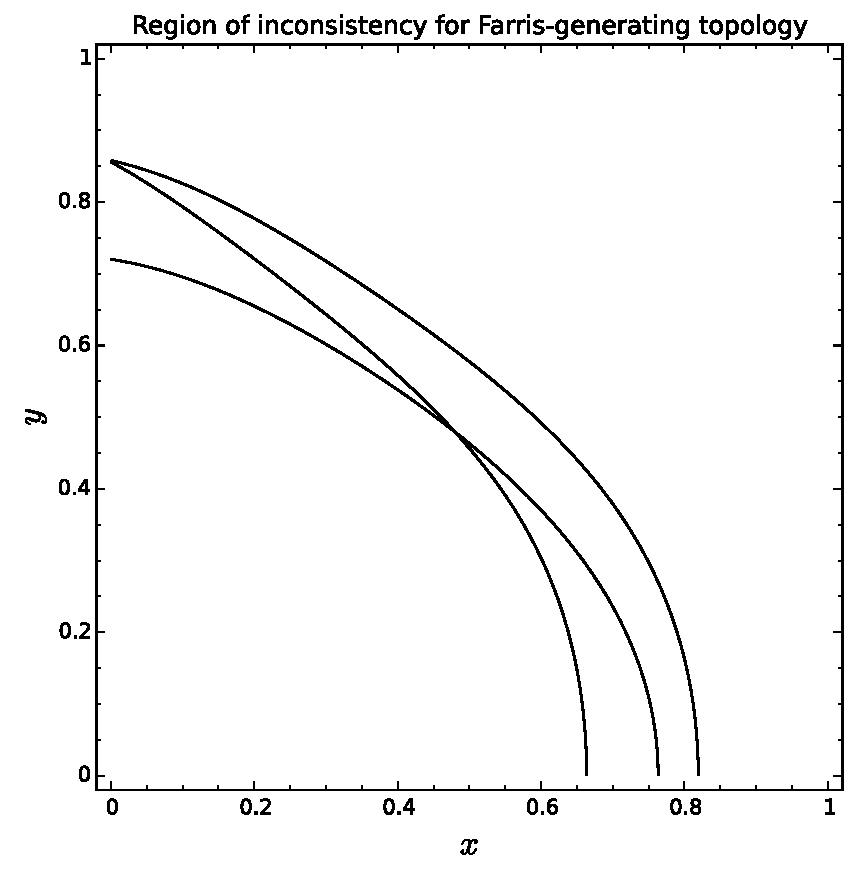
\includegraphics[width=.9\textwidth]{analytic-inconsistency}
\caption{
    Regions of inconsistency.
    Due to the looseness of the upper and lower bounds, the parameters in the top right do not necessarily indicate consistency, though all parameters in the labeled region will result in an inconsistency.
}
\label{fig:inconsistency-farris}
\end{figure}

\paragraph{Examples}

See Table~\ref{tab:examples} for parameters, bounds and true likelihood values obtained via basin hopping.

Set $\{x, y\} = \{0.25, 0.25\}$.
For a Farris zone generating topology, we have
$$
L^{p,1}_{\tau_1,\tau_1}(\mathbf{a}_{xy}) \approx -2.17803560694157,
$$
$$
L^{p,2}_{\tau_1,\tau_1}(\mathbf{a}_{xy}) \approx -2.17803560694157
$$
and
$$
L^{p,3}_{\tau_1,\tau_1}(\mathbf{a}_{xy}) \approx -2.17803560694157.
$$
Computing the upper bound yields
$$
\max_{t,\fullAncestralStateCategories} \ \ell_{\tau_1,\{x,y,y\}}(\fullAncestralStateCategories,\tau_1,t) \le -4.22274479428471
$$
and it remains to show that
$$
\max_{t,\fullAncestralStateCategories} \ \ell_{\tau_1,\{x,y,y\}}(\fullAncestralStateCategories,\tau_2,t) \ge -4.22274479428471.
$$

For the same generating parameters,
$$
d_{xy} = 0.498046875, \ e_{xy} = 0.2431640625,
$$
resulting in
$$
L^{p,1}_{\tau_1,\tau_2}(d_{xy},e_{xy}) \approx -2.07968569223991
$$
and
$$
h_{\tau_1,\{x,y,y\}}(\tau_2,\{1, 1-d_{xy}-2e_{xy}, 0\}) \approx -2.07748833719921.
$$
The lower bound in this case becomes
$$
\max_{t,\fullAncestralStateCategories} \ \ell_{\tau_1,\{x,y,y\}}(\fullAncestralStateCategories,\tau_2,t) \ge -4.15717402943912
\ge -4.22274479428471 \ge \max_{t,\fullAncestralStateCategories} \ \ell_{\tau_1,\{x,y,y\}}(\fullAncestralStateCategories,\tau_1,t)
$$
where site patterns are generated from the Farris zone topology.
Confirming, run \texttt{python}'s numerical optimization solver for $\{.25, .25\}$.
Since we are computing a constrained maximization, we can find a global maximum using basin hopping, and doing so yields
$$
\max_{t,\fullAncestralStateCategories} \ \ell_{\tau_1,\{x,y,y\}}(\fullAncestralStateCategories,\tau_1,t) \approx -4.5101771294218045
$$
and
$$
\max_{t,\fullAncestralStateCategories} \ \ell_{\tau_1,\{x,y,y\}}(\fullAncestralStateCategories,\tau_2,t) \approx -4.1544859851260281.
$$
It looks like the lower bound is tighter than the upper bound, so we may try focusing there.

\section{Discussion}

Neyman-Scott paradox.

Interesting that here we are simulating on the Farris tree and end up with the Felsenstein tree.
For maximum parsimony it's the opposite \cite{Felsenstein1978-rr}.
Discussion of number of parameters of each.

However, note that \cite{Siddall1998-hq} get things going the same way, although \cite{Swofford2001-hr} show that the problem is that they didn't simulate long enough sequences.

\bibliographystyle{plain}
\bibliography{joint_inf}

\end{document}
